% 9 variables in here:
% h_1 = 10.0, h_2 = 10.0, h_3 = 12.0, ux_1 = 0.0, ux_2 = 0.0, ux_3 = 0.0, uy_1 = 0.0, uy_2 = 0.0, uy_3 = 0.0
\begin{figure}[h!]
\centering
  \subfigure[] {
    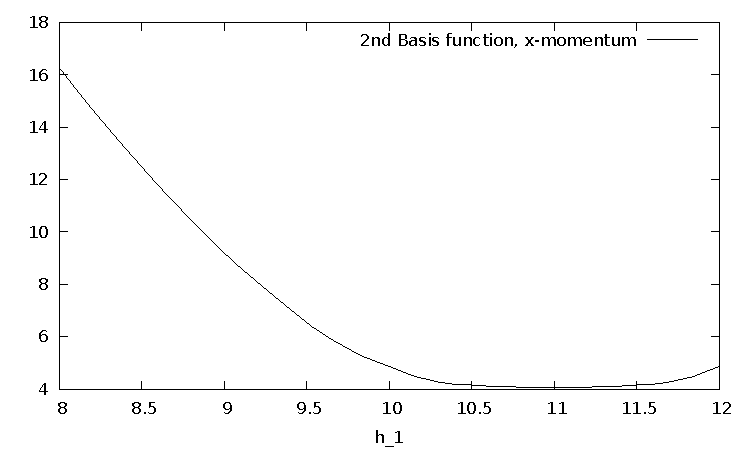
\includegraphics[scale=\zoomfactor]{{{ord1_differing_h2_h3_10_12/y_10.0_12.0_0.0_0.0_0.0_0.0_0.0_0.0f2}}}
  }
  \subfigure[] {
    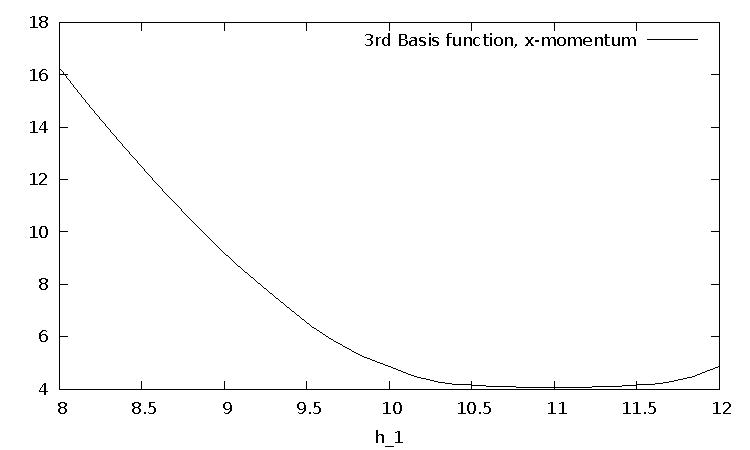
\includegraphics[scale=\zoomfactor]{{{ord1_differing_h2_h3_10_12/y_10.0_12.0_0.0_0.0_0.0_0.0_0.0_0.0f4}}}
  }
\caption{Errors in $x$-momentum for second and third basis function. All momentums are set to 0, $h_2=10$ and $h_3=12$.}
\label{fig:stiffneses-analysis-ord1-h2-10-h3-12}
\end{figure}
